\section{はじめに}
生物の細胞には様々な機能が備わっている.
まず,細胞は分裂して自分のコピーを作り出すことができる.
また,多細胞生物の場合,細胞は周囲の状況から自分の役割を認識し,それに特化した細胞に分化することがある.
ほかにも,大腸菌やゾウリムシなどの場合,べん毛や繊毛を振り回して水中を泳ぐことができる.

こうした機能は決して天から降ってきたものではなく,細胞内の化学反応によって綿密に制御されている.
一般に細胞は,何らかの物質(リガンド)の濃度を感知し,それに応じて適切に振る舞いを制御している.
ここで,リガンドの濃度を感知するため,細胞はリガンドと結合する部分(サイト)を持つ受容体を用いる.
つまり,リガンドが多いほど受容体のサイトはリガンドで埋まっていくはずなので,逆に受容体のサイトがどれだけ埋まっているか(占有率)をもとにリガンドの濃度を知ることができる.
受容体のサイトの占有率は,受容体とリガンドの複合体から発される信号や,受容体が酵素として働く反応への影響などを通して,細胞の振る舞いを変化させる.

では,リガンドの濃度と受容体のサイトの占有率の関係は具体的にどうなっているのだろうか.
本稿では,参考文献\cite{TBoC}をもとに,リガンドと受容体の結合の仕方を3通り考える.
そしてその各々について,数式を用いて定量的に議論する.

\section{最も単純な反応}
まず,受容体Yが1つだけ結合サイトを持ち,そこにリガンドXが結合する場合を考える.
このときの化学反応式は
\begin{equation}
  \ce{X + Y <=>[$k$_{on}][$k$_{off}] XY}
\end{equation}
となる.
ここで,矢印の上についている文字は正反応(左から右への反応)の速度定数を表し,矢印の下についている文字は逆反応(右から左への反応)の速度定数を表す.
この反応のレート方程式は,
\begin{equation}
  \dv{t}[\ce{XY}] = k_{\mathrm{on}}[\ce{X}][\ce{Y}] - k_{\mathrm{off}}[\ce{XY}]
\end{equation}
となる.
定常状態ではどの物質の濃度も変化しなくなるので,上式の左辺は0となる.
したがって
\begin{equation}
  \frac{[\ce{X}][\ce{Y}]}{[\ce{XY}]} = \frac{k_{\mathrm{off}}}{k_{\mathrm{on}}}
\end{equation}
を得る.
この量は解離定数と呼ばれる定数である:
\begin{equation}
  K_d = \frac{k_{\mathrm{off}}}{k_{\mathrm{on}}}
\end{equation}
ここで受容体分子の総濃度を
\begin{equation}
  [\ce{Y_{total}}] = [\ce{Y}] + [\ce{XY}]
\end{equation}
とし,これを一定と見なす.
すると,受容体の結合サイトの占有率$p$は
\begin{equation}
  p = \frac{[\ce{XY}]}{[\ce{Y_{total}}]} = \frac{[\ce{X}]}{K_d + [\ce{X}]} \label{normal}
\end{equation}
と分かる.

\begin{figure}[htbp]
  \centering
  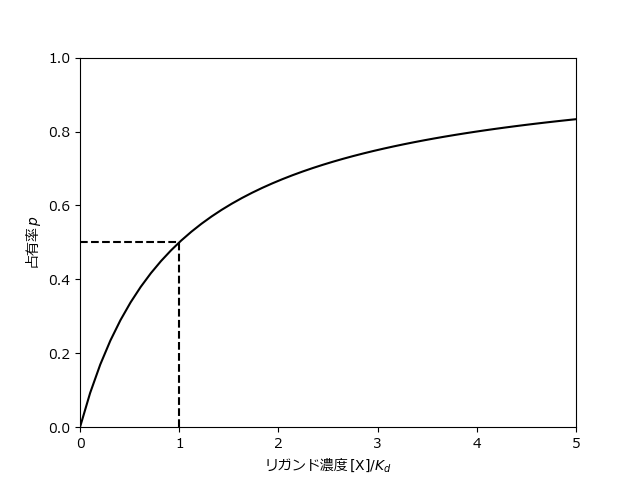
\includegraphics[width=10cm]{simple.png}
  \caption{最も単純なモデルで得られる曲線}
  \label{fig:simple}
\end{figure}

この式\eqref{normal}をプロットしてみると,図\ref{fig:simple}のような双曲線が得られる.
この図から,リガンド濃度が増えると受容体は埋まっていき,占有率が頭打ちになっていく(飽和する)ことが分かる.
